\documentclass{article}%
\usepackage{amsmath, amsthm, amssymb, amsfonts, float, graphicx,
wasysym, latexsym, amstext, eucal, verbatim}%
\usepackage{amsmath}%
\setcounter{MaxMatrixCols}{30}%
\usepackage{amsfonts}%
\usepackage{amssymb}%
\usepackage{graphicx}
%TCIDATA{OutputFilter=latex2.dll}
%TCIDATA{Version=5.00.0.2606}
%TCIDATA{LastRevised=Friday, February 26, 2010 11:54:11}
%TCIDATA{<META NAME="GraphicsSave" CONTENT="32">}
%TCIDATA{<META NAME="SaveForMode" CONTENT="1">}
%TCIDATA{BibliographyScheme=Manual}
\oddsidemargin 0.0in
\textwidth 6.5in
\begin{document}

%\title{}
%\author{}
%\maketitle


\renewcommand{\qedsymbol}{\smiley}

\begin{description}


\item[convex hinge]  Given a hinge, the boundary of the hinge forms a
quadrilateral. If all the interior angles of this quadrilateral are less than
or equal to $\pi$ (radians) then the hinge is called a \emph{convex hinge}.

\item[Delaunay triangulation]  If all the hinges of a triangulation are
Delaunay hinges, then the triangulation is called a Delaunay triangulation.

\item[dual edge]  Given a triangle $\{i,j,k\}$ in a triangulation with no
weights, we consider the perpendicular bisector of each edge. These bisectors
intersect at a single point. We call the line segment that extends from an
edge to this point of intersection, the dual of that edge.********

%%pic


\item[flip]  A flip of an edge (or hinge) is an action that changes triangles
in the triangulation. The typical flip in $2$ dimensions (a $2-2$ flip)
switches between two decompositions of a quadrilateral into two triangles.
That is the triangles $\{h,i,j\}$ and $\{i,j,k\}$ flip to become $\{h,k,i\}$
and $\{h,k,j\}$. We say that the edge $\{i,j\}$ flips to become $\{h,k\}.$
\begin{figure}[ptbh]
\centering
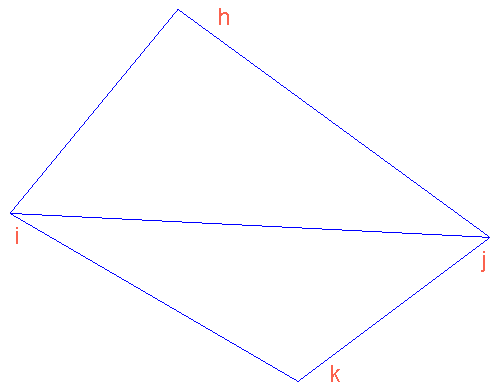
\includegraphics[height=.8in]{convex_hinge_nondelaunay.pdf}
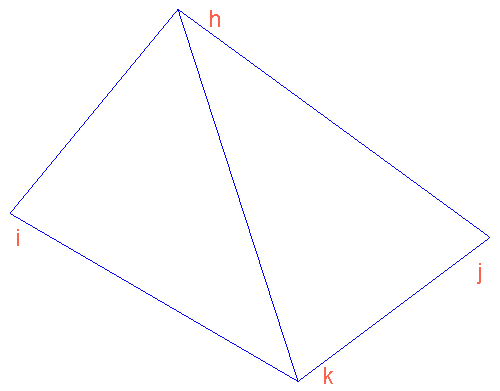
\includegraphics[height=.8in]{convex_hinge_delaunay.pdf}   \caption{before and
after flip}%
\label{fig:convex_hinge_nondelaunay}%
\end{figure}

\item[flip algorithm] 

\item[hinge]  A hinge is a pair of triangles that share an edge. We often
denote a hinge using the vertices of the triangles, for example $\{h,i,j\}$
and $\{i,j,k\}$ are faces that share the edge $\{i,j\}$ and so together they
form a hinge. In a two-dimensional manifold, a (non-boundary) edge determines
a unique hinge, for example $\{i,j\}$ determines the hinge formed by
$\{h,i,j\}$ and $\{i,j,k\}$. An important point is that a triangle may have
duplicate edges or vertices, and so a hinge being constructed of triangles can
also have duplicate edges or vertices. In this case, we would need to denote a
hinge by $\left\{  f_{1},f_{2},e\right\}  ,$ where $f_{1}$ and $f_{2}$ are
triangles, and $e$ is an edge local to both $f_{1}$ and $f_{2}.$

\item[nonconvex hinge]  A hinge which is not convex is a \emph{nonconvex
hinge}. An important characteristic of such a hinge is that the line between
the vertices that are not adjacent to the identifying edge, lies outside the
hinge. These hinges cannot flip (geometrically) in the usual way.

\item[weighted triangulation]  Given a piece flat triangulation we can assign
a weight to each vertex of the triangulation. Each weight can be thought of as
a radius of a circle around the vertex it is assigned to. A triangulation with
weights assigned to the vertices is called a weighted triangulation. 

\item[weighted Delaunay triangulation]  If all the hinges in a weighted
triangulation are weighted Delaunay hinges, then the weighted triangulation is
called a weighted Delaunay triangulation.

\item[weighted Voronoi diagram]  A weighted Voronoi diagram is all of the dual
cells of a weighted Delaunay triangulation.
\end{description}


\end{document}